\chapter{Results}

The results will include three parts. 
First, the performance of rCOMMIT will be visualized from different angles. Second, the performance of the models based on the 
pseudo ground truth will be shown. Last, a comparison between the results from COMMIT and SIFT is conducted.

\section{Performance of rCOMMIT}

Fig \ref{fig:heatmap} shows the distribution of ARs in different subset sizes on three subjects, 
and table \ref{table:cate} indicates the values and the ranges of categories in the figure. 

Adding the distribution ratio in category 0 and 6, it shows that more than 50\% of the streamlines
receive either 0\% AR or 100\% AR after rCOMMIT for all the subsets. For the data of 10 million size, all the streamlines
are divided into category 0 and 6, so there is no value in the other groups. Because running COMMIT multiple times on the same data gives back the same results for each streamline. 
When applying COMMIT to the smaller datasets, the ratio of streamlines from 
category 1 to 5 increases. Meanwhile, the ratio of streamlines with AR = 100\% increases from 7.0\% to 28.5\%,
while the streamlines with AR = 0\% decreases largely, from 93.4\% to 27.2\%.


\begin{table}[]
    \resizebox{\textwidth}{!}{%
    \begin{tabular}{|c|c|c|c|c|c|c|c|}
    \hline
    Category                                                                   & 0   & 1            & 2           & 3             & 4             & 5            & 6     \\ \hline
    \begin{tabular}[c]{@{}c@{}}Acceptance Rate(AR) \\ Range/Value\end{tabular} & 0\% & (0\%,20\%{]} & (20\%,40{]} & (40\%,60\%{]} & (60\%,80\%{]} & (80\%,100\%) & 100\% \\ \hline
    \end{tabular}%
    }
    \caption{The values and ranges of different acceptance rate categories. For category 0, the AR is 0\%.
    For category 6, the AR is 100\%. For the other categories, the ARs are classified by the ranges. These intervals 
    do not include the lower bound and include the higher bound, except category 5 which exclues both 80\% and 100\%.}
    \label{table:cate}
\end{table}

\begin{figure}[ht]
    \centering
    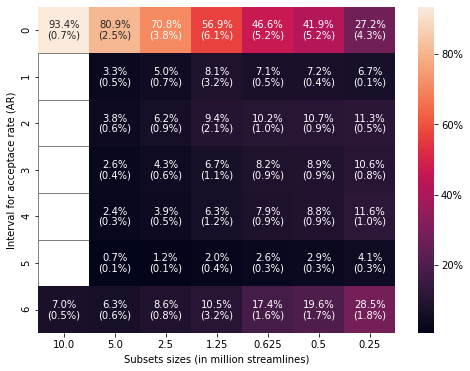
\includegraphics[width= 15cm]{figures/heatmap.png}
        \caption{The distribution of acceptance rates in different subset sizes. Each cell includes the mean ratio of 
        the streamlines across subjects and the standard deviations in the parentheses. In the column of the 10 million data, there is no value from category 1 to 5.
        }
    \label{fig:heatmap}
\end{figure}

\begin{figure}[ht]
    \centering
    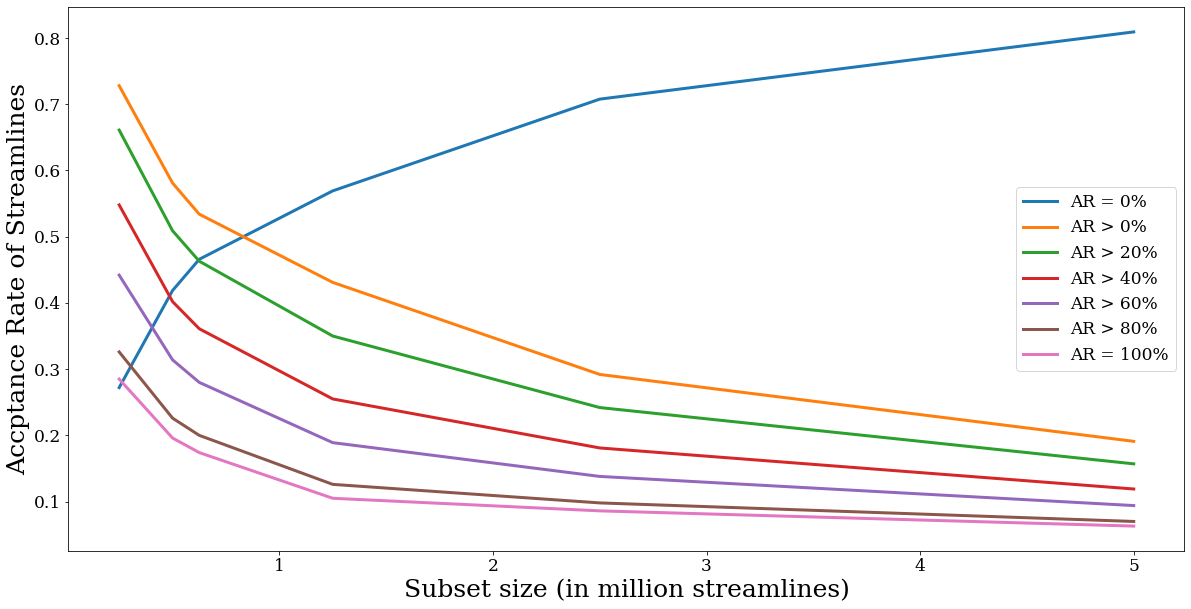
\includegraphics[width= 15cm]{figures/ARplot.png}
        \caption{The changes of acceptance rate from rCOMMIT with different subset size.
        The curves show the averaged AR over subjects. As shown, the ARs of streamlines get higher in the smaller
        subsets.}
    \label{fig:ARplot}
\end{figure}

\subsection{Pseudo Ground Truth}

\begin{figure}[ht]
    \centering
    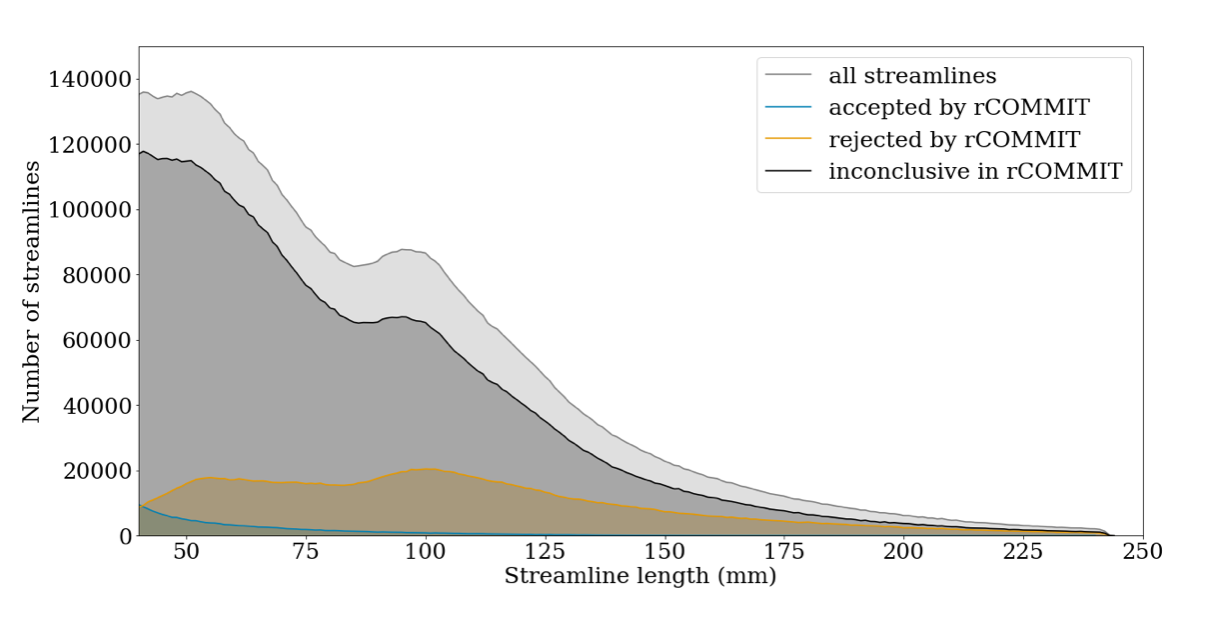
\includegraphics[width= 15cm]{figures/three_groups_hist.png}
        \caption{The distribution of streamlines from one exemplary subject with respect to the length in three groups: plausible group, implausible group and inconclusive group. }
    \label{fig:threegroup}
\end{figure}

\section{Model Classification}

\section{Comparison Between rCOMMIT and rSIFT}

\subsection{Performance between methods}

\subsection{Results from rCOMMIT and rSIFT}

\begin{table}[]
    \centering
    \resizebox{\columnwidth}{!}{%
    \begin{tabular}{|cc|cc|cc|cc|cc|}
    \hline
    \multicolumn{2}{|c|}{Groups} &
      \multicolumn{2}{c|}{Plausible Group} &
      \multicolumn{2}{c|}{Intersection} &
      \multicolumn{2}{c|}{Implausible Group} &
      \multicolumn{2}{c|}{Intersection} \\ \hline
    \multicolumn{2}{|c|}{Methods} &
      \multicolumn{1}{c|}{rCOMMIT} &
      rSITF &
      \multicolumn{1}{c|}{rCOMMIT} &
      rSITF &
      \multicolumn{1}{c|}{rCOMMIT} &
      rSITF &
      \multicolumn{1}{c|}{rCOMMIT} &
      rSITF \\ \hline
    \multicolumn{1}{|c|}{Number of streamlines} &
      \multirow{2}{*}{Subject 1} &
      \multicolumn{1}{c|}{475 959} &
      146 252 &
      \multicolumn{2}{c|}{89 052} &
      \multicolumn{1}{c|}{1 663 161} &
      5 263 290 &
      \multicolumn{2}{c|}{1 486 537} \\ \cline{1-1} \cline{3-10} 
    \multicolumn{1}{|c|}{Percentage} &
       &
      \multicolumn{1}{c|}{4,76 \%} &
      1,46 \% &
      \multicolumn{1}{c|}{18,71 \%} &
      60,89 \% &
      \multicolumn{1}{c|}{16,63 \%} &
      52,63 \% &
      \multicolumn{1}{c|}{89,38 \%} &
      28,24 \% \\ \hline
    \multicolumn{1}{|c|}{Number of streamlines} &
      \multirow{2}{*}{Subject 3} &
      \multicolumn{1}{c|}{215 796} &
      170 814 &
      \multicolumn{2}{c|}{62 376} &
      \multicolumn{1}{c|}{1 970 751} &
      5 445 176 &
      \multicolumn{2}{c|}{1 813 401} \\ \cline{1-1} \cline{3-10} 
    \multicolumn{1}{|c|}{Percentage} &
       &
      \multicolumn{1}{c|}{2,16 \%} &
      1,71 \% &
      \multicolumn{1}{c|}{28,91 \%} &
      36,52 \% &
      \multicolumn{1}{c|}{19,71 \%} &
      54,45 \% &
      \multicolumn{1}{c|}{92,02 \%} &
      33,30 \% \\ \hline
    \multicolumn{1}{|c|}{Number of streamlines} &
      \multirow{2}{*}{Subject 3} &
      \multicolumn{1}{c|}{379 458} &
      176 320 &
      \multicolumn{2}{c|}{88 715} &
      \multicolumn{1}{c|}{2 581 409} &
      5 195 768 &
      \multicolumn{2}{c|}{2 215 674} \\ \cline{1-1} \cline{3-10} 
    \multicolumn{1}{|c|}{Percentage} &
       &
      \multicolumn{1}{c|}{3,79 \%} &
      1,76 \% &
      \multicolumn{1}{c|}{23,38 \%} &
      50,31 \% &
      \multicolumn{1}{c|}{25,81 \%} &
      51,96 \% &
      \multicolumn{1}{c|}{85,83 \%} &
      42,64 \% \\ \hline
    \end{tabular}%
    }
    \end{table}





\begin{figure}[ht]
    \centering
    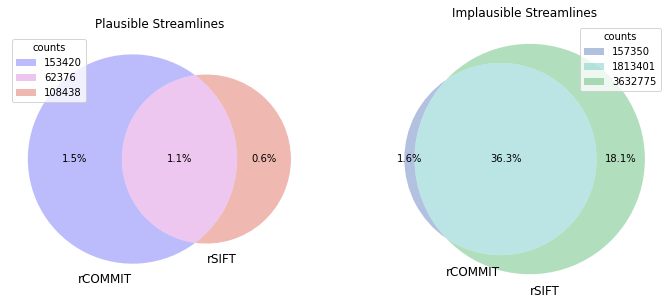
\includegraphics[width= 15cm]{figures/comp_s_c.png}
        \caption{The distribution of streamlines from one exemplary subject with respect to the length in three groups: plausible group, implausible group and inconclusive group. }
    \label{fig:com_s_c}
\end{figure}


Describe the results of the degree project.
